\documentclass[12pt,twoside]{article}
%%%%%%%%%%%%%%%%%%%%%%%%%%%%%%%%%%%%%%%%%%%%%%%%%%%%%%%%%%%%%
% Meta informations:
\newcommand{\trauthor}{Daniel Speck und Florian Kock}
\newcommand{\trtype}{Praktikum Paper} %{Seminararbeit} %{Proseminararbeit}
\newcommand{\trcourse}{Dokumentation der erstellten Applikation}
\newcommand{\trtitle}{Pong, gespielt von KNNs}
\newcommand{\trmatrikelnummer}{6321317 6346646}
\newcommand{\tremail}{2speck@informatik.uni-hamburg.de, 2kock@informatik.uni-hamburg.de}
\newcommand{\trarbeitsbereich}{Knowledge Technology, WTM}
\newcommand{\trdate}{\today}

%%%%%%%%%%%%%%%%%%%%%%%%%%%%%%%%%%%%%%%%%%%%%%%%%%%%%%%%%%%%%
% Languages:

% Falls die Ausarbeitung in Deutsch erfolgt:
 \usepackage[german]{babel}
 \usepackage[T1]{fontenc}
 \usepackage{german}
% \usepackage[latin1]{inputenc}
% \usepackage[latin9]{inputenc}	 				
 \selectlanguage{german}
 
 %\usepackage[latin1]{inputenc}
\usepackage[utf8]{inputenc}

% If the thesis is written in English:
%\usepackage[english]{babel} 						
%\selectlanguage{english}

%%%%%%%%%%%%%%%%%%%%%%%%%%%%%%%%%%%%%%%%%%%%%%%%%%%%%%%%%%%%%
% Bind packages:
\usepackage{hyperref}
\usepackage{acronym}                    % Acronyms
\usepackage{algorithmic}								% Algorithms and Pseudocode
\usepackage{algorithm}									% Algorithms and Pseudocode
\usepackage{amsfonts}                   % AMS Math Packet (Fonts)
\usepackage{amsmath}                    % AMS Math Packet
\usepackage{amssymb}                    % Additional mathematical symbols
\usepackage{amsthm}
\usepackage{booktabs}                   % Nicer tables
%\usepackage[font=small,labelfont=bf]{caption} % Numbered captions for figures
\usepackage{color}                      % Enables defining of colors via \definecolor
\definecolor{uhhRed}{RGB}{254,0,0}		  % Official Uni Hamburg Red
\definecolor{uhhGrey}{RGB}{122,122,120} % Official Uni Hamburg Grey
\usepackage{fancybox}                   % Gleichungen einrahmen
\usepackage{fancyhdr}										% Packet for nicer headers
%\usepackage{fancyheadings}             % Nicer numbering of headlines

%\usepackage[outer=3.35cm]{geometry} 	  % Type area (size, margins...) !!!Release version
%\usepackage[outer=2.5cm]{geometry} 		% Type area (size, margins...) !!!Print version
%\usepackage{geometry} 									% Type area (size, margins...) !!!Proofread version
\usepackage[outer=3.15cm]{geometry} 	  % Type area (size, margins...) !!!Draft version
\geometry{a4paper,body={5.8in,9in}}

\usepackage{graphicx}                   % Inclusion of graphics
%\usepackage{latexsym}                  % Special symbols
\usepackage{longtable}									% Allow tables over several parges
\usepackage{listings}                   % Nicer source code listings
\usepackage{multicol}										% Content of a table over several columns
\usepackage{multirow}										% Content of a table over several rows
\usepackage{rotating}										% Alows to rotate text and objects
\usepackage[hang]{subfigure}            % Allows to use multiple (partial) figures in a fig
%\usepackage[font=footnotesize,labelfont=rm]{subfig}	% Pictures in a floating environment
\usepackage{tabularx}										% Tables with fixed width but variable rows
\usepackage{url,xspace,boxedminipage}   % Accurate display of URLs

%%%%%%%%%%%%%%%%%%%%%%%%%%%%%%%%%%%%%%%%%%%%%%%%%%%%%%%%%%%%%
% Configurationen:

\hyphenation{whe-ther} 									% Manually use: "\-" in a word: Staats\-ver\-trag

%\lstloadlanguages{C}                   % Set the default language for listings
\DeclareGraphicsExtensions{.pdf,.svg,.jpg,.png,.eps} % first try pdf, then eps, png and jpg
\graphicspath{{./src/}} 								% Path to a folder where all pictures are located
\pagestyle{fancy} 											% Use nicer header and footer

% Redefine the environments for floating objects:
\setcounter{topnumber}{3}
\setcounter{bottomnumber}{2}
\setcounter{totalnumber}{4}
\renewcommand{\topfraction}{0.9} 			  %Standard: 0.7
\renewcommand{\bottomfraction}{0.5}		  %Standard: 0.3
\renewcommand{\textfraction}{0.1}		  	%Standard: 0.2
\renewcommand{\floatpagefraction}{0.8} 	%Standard: 0.5

% Tables with a nicer padding:
\renewcommand{\arraystretch}{1.2}

%%%%%%%%%%%%%%%%%%%%%%%%%%%%
% Additional 'theorem' and 'definition' blocks:
\theoremstyle{plain}
\newtheorem{theorem}{Theorem}[section]
%\newtheorem{theorem}{Satz}[section]		% Wenn in Deutsch geschrieben wird.
\newtheorem{axiom}{Axiom}[section] 	
%\newtheorem{axiom}{Fakt}[chapter]			% Wenn in Deutsch geschrieben wird.
%Usage:%\begin{axiom}[optional description]%Main part%\end{fakt}

\theoremstyle{definition}
\newtheorem{definition}{Definition}[section]

%Additional types of axioms:
\newtheorem{lemma}[axiom]{Lemma}
\newtheorem{observation}[axiom]{Observation}

%Additional types of definitions:
\theoremstyle{remark}
%\newtheorem{remark}[definition]{Bemerkung} % Wenn in Deutsch geschrieben wird.
\newtheorem{remark}[definition]{Remark} 

%%%%%%%%%%%%%%%%%%%%%%%%%%%%
% Provides TODOs within the margin:
\newcommand{\TODO}[1]{\marginpar{\emph{\small{{\bf TODO: } #1}}}}

%%%%%%%%%%%%%%%%%%%%%%%%%%%%
% Abbreviations and mathematical symbols
\newcommand{\modd}{\text{ mod }}
\newcommand{\RS}{\mathbb{R}}
\newcommand{\NS}{\mathbb{N}}
\newcommand{\ZS}{\mathbb{Z}}
\newcommand{\dnormal}{\mathit{N}}
\newcommand{\duniform}{\mathit{U}}

\newcommand{\erdos}{Erd\H{o}s}
\newcommand{\renyi}{-R\'{e}nyi}
%%%%%%%%%%%%%%%%%%%%%%%%%%%%%%%%%%%%%%%%%%%%%%%%%%%%%%%%%%%%%
% Document:
\begin{document}
\renewcommand{\headheight}{14.5pt}

\fancyhead{}
\fancyhead[LE]{ \slshape \trauthor}
\fancyhead[LO]{}
\fancyhead[RE]{}
\fancyhead[RO]{ \slshape \trtitle}

%%%%%%%%%%%%%%%%%%%%%%%%%%%%
% Cover Header:
\begin{titlepage}
	\begin{flushleft}
		Universit\"at Hamburg\\
		Department Informatik\\
		\trarbeitsbereich\\
	\end{flushleft}
	\vspace{3.5cm}
	\begin{center}
		\huge \trtitle\\
	\end{center}
	\vspace{3.5cm}
	\begin{center}
		\normalsize\trtype\\
		[0.2cm]
		\Large\trcourse\\
		[1.5cm]
		\Large \trauthor\\
		[0.2cm]
		\normalsize Matr.Nr. \trmatrikelnummer\\
		[0.2cm]
		\normalsize\tremail\\
		[1.5cm]
		\Large \trdate
	\end{center}
	\vfill
\end{titlepage}

	%backsite of cover sheet is empty!
\thispagestyle{empty}
\hspace{1cm}
\newpage

%%%%%%%%%%%%%%%%%%%%%%%%%%%%
% Abstract:

% Abstract gives a brief summary of the main points of a paper:
\section*{Abstrakt}

Unsere Aufgabe des letzten Semesters war es, in dem Praktikum Neuronale Netze eine Aufgabe zu lösen. Wir haben uns für das, in den 70ern populäre Spiel, Pong entschieden. 
Dieses war dahingehend interessant, da es gleich mehrere Probleme zu lösen gab:
  \begin{itemize}
  \item die Zeitverzögerte Bewertung
  \item das erkennen der Flugrichtung durch Rekurrenz
\end{itemize}



\begin{quote}
Das Spielprinzip von Pong ist simpel und ähnelt dem des Tischtennis: Ein Punkt („Ball“) bewegt sich auf dem Bildschirm hin und her. Jeder der beiden Spieler steuert einen senkrechten Strich („Schläger“), den er mit einem Drehknopf (Paddle) nach oben und unten verschieben kann. Lässt man den „Ball“ am „Schläger“ vorbei, erhält der Gegner einen Punkt. 
(Wikipedia)
\end{quote}

Im Anschließenden werden wir die Grundlagen unseres Programmes beschreiben.



% Lists:
\setcounter{tocdepth}{2} 					% depth of the table of contents (for Seminars 2 is recommented)
\tableofcontents
\pagenumbering{arabic}


%%%%%%%%%%%%%%%%%%%%%%%%%%%%
% Content:

% the actual content, usually separated over a number of sections
% each section is assigned a label, in order to be able to put a
% crossreference to it

\section{Vorbedingungen und Anforderungen}

Um die Applikation erfolgreich ausführen zu können sind folgende Anforderungen an die Laufzeitumgebung notwendig:


\begin{itemize}
\item Python3.4
\begin{centering}
\includegraphics[width=0.3\textwidth]{python-logo-master-v3-TM.png}
\end{centering}
\item NumPy
\begin{centering}
\includegraphics[width=0.3\textwidth]{NumPy_logo.png}
\end{centering}
\item The Python Standard Library 
\begin{itemize}
 \item multiprocessing
 \item threading
 \item sys
 \item random
 \item os.path
 \item logging
 \item json
 \item socketserver
 \item tkinter
 \item socket
 \item time
 \item datetime
 \item copy
 
 
\end{itemize} 

\end{itemize} 
 
 

\section{Schnelleinstieg}

Der Schnelleinstieg führt über folgende Befehle: (Wenn die Vorbedingungen gegeben sind!)


Starten des Hauptprogramms: 
\begin{lstlisting}[frame=single,language=bash]  % Start your code-block

> ls
__init__.py	 knnframe.py 	telegramframe.py
__pycache__	 main.py		    visu.py
concol.py	 recneunet.py
court.py	 save
> python3.4 main.py 
... starting application ...
\end{lstlisting}

Starten der Visualisierung zum Hauptprogramm:
\begin{lstlisting}[frame=single,language=bash]  % Start your code-block

> ls
__init__.py	 knnframe.py	  telegramframe.py
__pycache__	 main.py		  visu.py
concol.py	 recneunet.py
court.py	 save
> python3.4 visu.py 
... starting visualisation ...
\end{lstlisting}


\section{Aufbau der Applikation}

Unsere Applikation ist in mehrere Datein und Module aufgeteilt. In der Abbildung~\ref{fig:ApplicationArchitecture} auf Seite~\pageref{fig:ApplicationArchitecture} ist die Grundstruktur zu erkennen. Die einzelnen Module werden unterschieden in die Haupt-Anwendung (main.py) \ref{main.py} und die Visualisierung (visu.py) \ref{visu.py}.  

\begin{figure}[hbtp]
	 \centerline{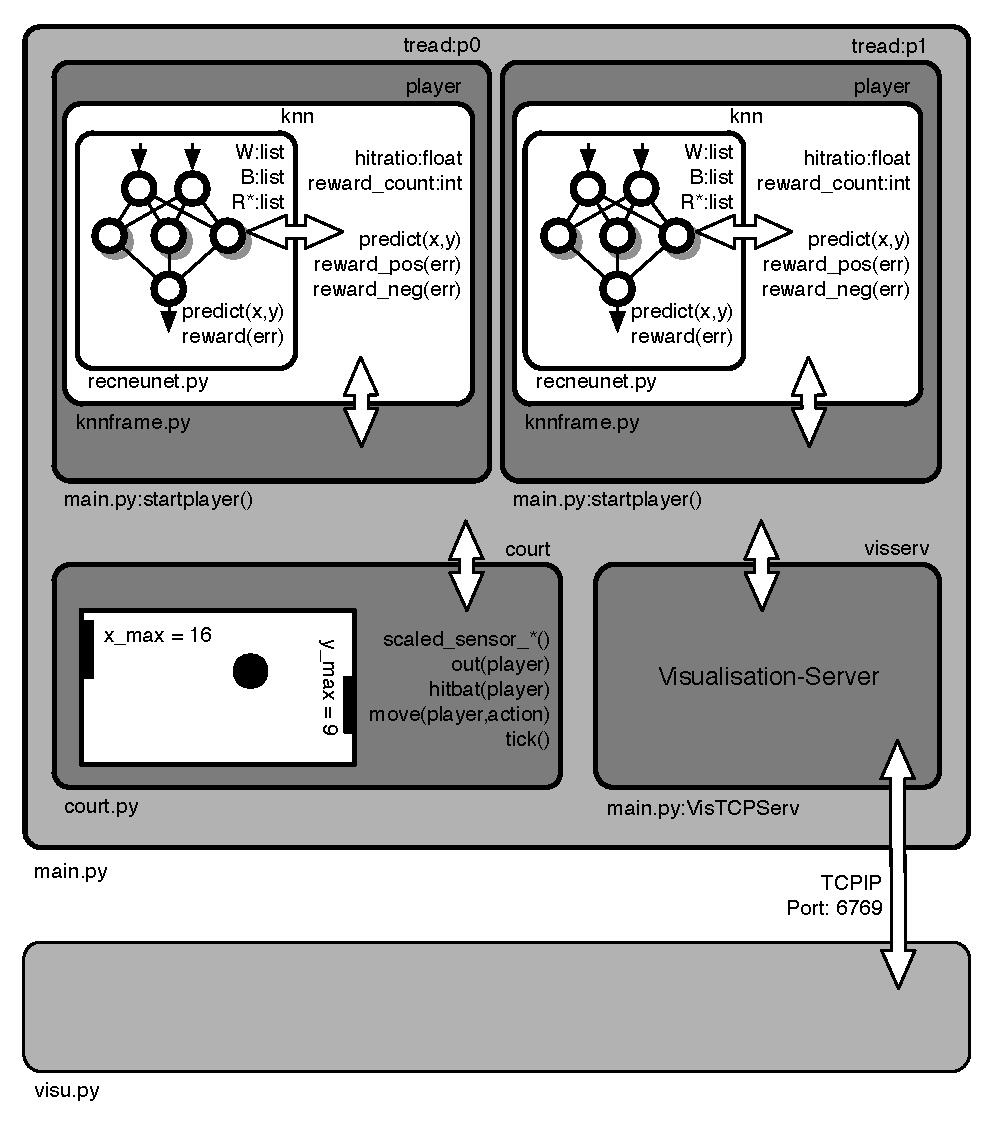
\includegraphics[]{ApplicationArchitecture.pdf}}
	 {\caption{Schematischer Aufbau der Pong-Applikation}\label{fig:ApplicationArchitecture}}
\end{figure}


\subsection{Die Haupanwendung - main.py}
\label{main.py}

Die Hauptapplikation besteht im wesentlichen aus einer Hauptschleife, die die Spielzüge (im Quellcode 'Ticks' genannt) kontrolliert. Der relevante Teil befindet sich hierzu in der \textit{main.py} in den Zeilen von ca. 360 bis 460.

Sie liefert in jedem Spielzug vom Spielfeld (siehe \ref{curt.py}) die Ballpositionen an die Spieler (siehe \ref{knnframe.py}) um anschließend deren Aktion wieder dem Spielfeld zuzuführen.

\subsubsection{Die Haupanwendung - curt.py}
\label{curt.py}
Das Spielfeld implementiert eine Simulation der Spielumgebung. Diese besteht, aus zwei Schlägern und einem Ball in einem rechteckigen Rahmen. Bei jedem Aufruf von \textit{tick()} berechnet das Spielfeld den nächsten Zustand des Balles, hierbei wird ebenfalls geprüft, ob der er die Bande, den Rahmen, überschritten hat und korrigiert dies. Ein solcher Abprall ist der Physik nachempfunden ("Einfallswinkel = Ausfallswinkel").
Das Ziel des Spieles ist es, den Ball mit dem Schläger zurückzuspielen, gelangt der Ball jedoch über die Linie, bedeutet dies, das der Ball wieder in der Mitte gestartet wird. Hierfür ist die \textit{__initvectors()} zuständig. Sie initialisiert die 


\subsubsection{Die Haupanwendung - knnframe.py}
\label{knnframe.py}


\subsection{Die Visualisierung - visu.py}
\label{visu.py}

Die Visualisierung der dient der einfachen Diagnose, des Zustands der Hauptapplikation welche keine eigene Visualisierung bereitstellt. Die Verbindung geschieht über TCP/IP über den Port 6769 und ist aktuell nur vom localhost erreichbar.

TODO: Screenshot und erklärung der Funktionen! 




\section{Conclusion}


Your text here...





\section{remove this!}
\label{sec:concl}

\begin{lstlisting}[frame=single,language=Python]  % Start your code-block
def netw_communication(conn):
    nc = NetwCon()
    connected = False
    while not connected:
        print('Try to connect...')
        connected = nc.connect()
        if not connected:
            time.sleep(1)
    print('connected, lets go...')
\end{lstlisting}


\end{document}


